\section{multiaccess media}

% multiple channels?
    % everyone receives everything?
% start with simple model
\begin{frame}{multiaccess media}
    \begin{itemize}
    \item shared air for radio/light signals
    \item shared wires for electrical/light signals
    \item \ldots
    \vspace{.5cm}
    \item needs:
        \begin{itemize}
        \item way to tell what signals are for whom
        \item way to decide who `talks' when/where
        \end{itemize}
    \end{itemize}
\end{frame}

\begin{frame}{shared wires}
    \begin{itemize}
    \item used to be how Ethernet worked
        \begin{itemize}
        \item before Ethernet switches were ubiquitous
        \end{itemize}
    \item how cable Internet works
        \begin{itemize}
        \item shared line to many customers in area
        \item need to share
        \end{itemize}
    \item usually how fiber-to-the-home works
        \begin{itemize}
        \item ``passive optical network''
        \item connect multiple fibers optically
        \end{itemize}
    \end{itemize}
\end{frame}

\begin{frame}{multiple channels}
    \begin{itemize}
    \item can have multiple channels over single medium
    \item typically: radio or electrical signal or light frequencies
    \item sender/receiver separate channels electrically/optically
    \vspace{.5cm}
    \item to start: will worry about coordinating one chnanel
    \end{itemize}
\end{frame}

\begin{frame}{wireless spectrum}
    \begin{itemize}
    \item most useful radio spectrum \textit{licensed}
    \item gov't gives exclusive rights (within some region) to specific organizations/poeple 
        \begin{itemize}
        \item example: cellular, TV, satellite, air traffic control, etc.
        \end{itemize}
    \item a lot of computer networking uses \textit{unlicensed} bands
        \begin{itemize}
        \item use without specific permission allowed
        \item still limits on power, procedures to avoid interference
        \end{itemize}
    \end{itemize}
\end{frame}

\begin{frame}{selected unlicensed bands}
    \begin{itemize}
    \item approx. frequencies unlicensed in US (not everywhere)
    \vspace{.5cm}
    \item 902--928 MHz (802.15.4 (IoT focused))
    \item 2.4--2.5 GHz (802.15.4; 802.11b/g/n/ax/\ldots; bluetooth; microwave ovens)
    \item 5.15 GHz--5.25 GHz (802.11a/n/ac/ax/\ldots)
    \item 5.25 GHz--5.73 GHz (802.11a/n/ac/ax/\ldots; also weather radar)
        \begin{itemize}
        \item requires `dynamic frequency selection'
        \end{itemize}
    \item 5.73 GHz--5.85 GHz (802.11a/n/ac/ax/\ldots)
    \item 5.93 GHz--7.12 GHz (802.11ax/\ldots)
    \item 24.0-24.2 GHz
    \item 57--64 GHz
    \end{itemize}
\end{frame}



\subsection{collisions}
\begin{frame}{collisions}
    \begin{itemize}
    \item $N$ nodes try to transmit one channel at same time
    \item likely outcomes for some receiver:
    \vspace{.5cm}
    \item receiver gets garbage
        \begin{itemize}
        \item ``collision''
        \end{itemize}
    \item receiver receives 1 of the $N$ collisions
    \end{itemize}
\end{frame}



\section{transmitting in the blind}
% FIXME: collision 1.5 ms apart for 1ms packets
\usetikzlibrary{arrows.meta}
\begin{frame}{running example}
\begin{itemize}
    \item based on Abramson, ``The Aloha System---Another alternative for computer comunications'' (1970)
    \vspace{.5cm}
    \item suppose we have shared radio with nodes A1, A2, \ldots, A$n$ and B
    \vspace{.5cm}
    \item A1, A2, \ldots A$n$ are all trying to transmit to B
    \item takes 1 ms to send message
    \item and want to collectively send $k$ messages per second
        \begin{itemize}
        \item randomly spaced (exponential distribution)
        \end{itemize}
\end{itemize}
\end{frame}

\begin{frame}{some probability}
    \begin{itemize}
    \item exponential distribution with mean $\lambda$
        \begin{itemize}
        \item our model for when packets sent
        \item ``memoryless'' distribution
        \item knowing when last packet sent tells you nothing about next
        \item (yes, not realistic)
        \end{itemize}
    \vspace{.5cm}
    \item probability events occur $< K$ time units apart \\
    $1-e^{-\lambda K}$
    \end{itemize}
\end{frame}


\begin{frame}{quiet time to avoid collisions}
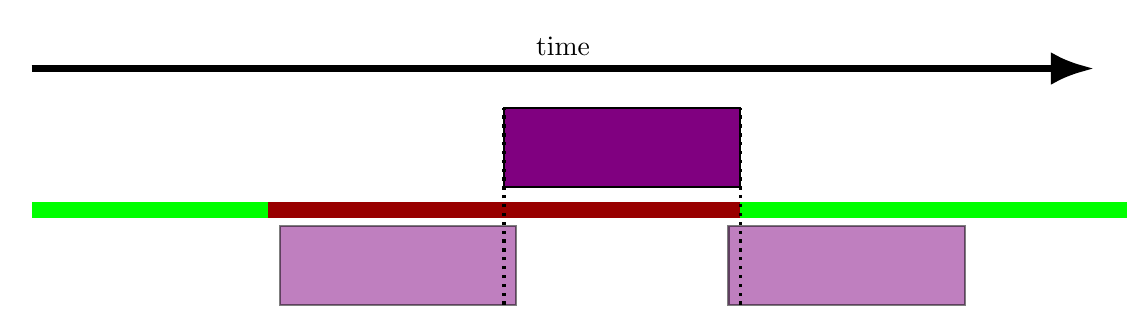
\begin{tikzpicture}
\begin{scope}[x=3cm]
    \draw[line width=1mm,-Latex] (-0.5, 0) -- (4, 0) node[above,midway] {time};
    \draw[thick,fill=violet] (1.5, -0.5) rectangle ++(1, -1);
    \draw[thick,fill=violet,opacity=0.5] (0.55, -2) rectangle ++(1, -1);
    \draw[thick,fill=violet,opacity=0.5] (2.45, -2) rectangle ++(1, -1);
    \path[fill=red!60!black] (0.5,-1.7) rectangle ++(2, -.2);
    \path[fill=green] (-0.5,-1.7) rectangle ++(1, -.2);
    \path[overlay,fill=green] (2.5,-1.7) rectangle ++(2, -.2);
    \draw[dotted,very thick] (1.5, -3) -- (1.5, -0.5);
    \draw[dotted,very thick] (2.5, -3) -- (2.5, -0.5);
\end{scope}
\end{tikzpicture}
\begin{itemize}
\item to avoid collision with 1 ms packet\ldots
\item can't start packet less than 1 ms before
\item can't start packet less than 1 ms after
\item $\rightarrow$ need 2 ms without packet starting for no collision
\end{itemize}
\end{frame}
% FIXME: diagram of 1.5 ms apart starts and collision

\begin{frame}{chance of collisions?(1)}
    \begin{itemize}
    \item to avoid collision when sending 1 ms packet
    \item need no other packet to be sent in 2ms period around its start time
    \vspace{.5cm}
    \item with $k$ packets/sec, chance is approx $1-e^{-\frac{2}{1000}k}$
    \end{itemize}
\end{frame}

\begin{frame}{chance of collision}
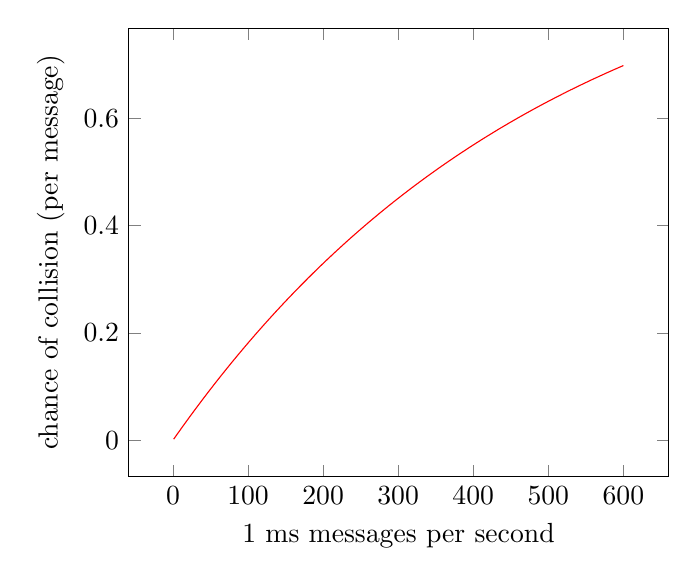
\begin{tikzpicture}
\begin{axis}[xlabel=1 ms messages per second,ylabel=chance of collision (per message)]
\addplot[domain=1:600,color=red,samples=1000]{1-exp(-(2 * x)/1000};
\end{axis}
\end{tikzpicture}
\end{frame}

\begin{frame}{retransmissions}
    \begin{itemize}
    \item what's going to happen when node can't send message
    \item probably it will retransmit it\ldots
    \vspace{.5cm}
    \item which means real transmission rate will be some $R > k$
        \begin{itemize}
        \item where $k$ is rate messages are generated
        \end{itemize}
    \item about $[1-e^{-2R\frac{1}{1000}}]$ chance of each message generated
    \item so $R = k + \left(1-e^{-2R\frac{1}{1000}}\right) \cdot R$
    \item $R = k + R - Re^{-2R\frac{1}{1000}}$
    \item $k = Re^{-2R\frac{1}{1000}}$
    \end{itemize}
\end{frame}

\begin{frame}{retranmissions (plot)}
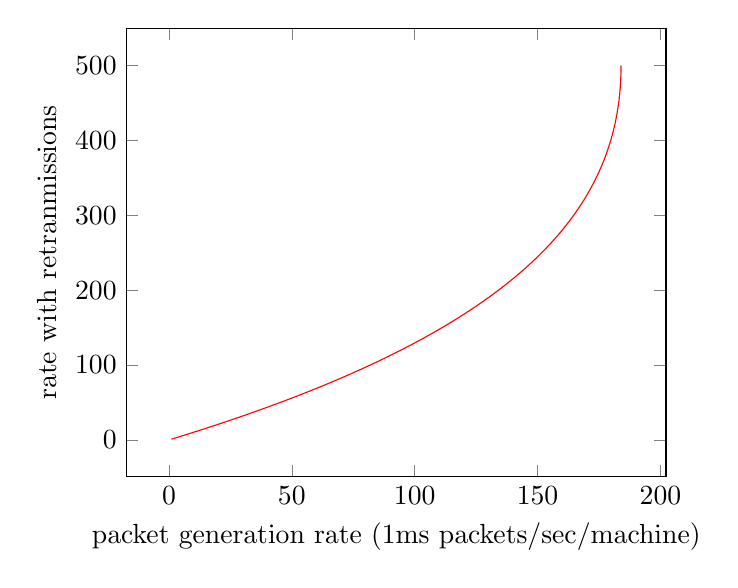
\begin{tikzpicture}
\begin{axis}[xlabel={packet generation rate (1ms packets/sec/machine)}, ylabel={rate with retranmissions}]
\addplot[domain=1:500,color=red,samples=1000] (x * exp(-2*x/1000), x);
\end{axis}
\end{tikzpicture}
\end{frame}

\begin{frame}{thinking about result}
    \begin{itemize}
    \item sending 500 1ms packet or retransmission/second
        \begin{itemize}
        \item using about half the capacity!
        \end{itemize}
    \item representing $\sim$ 186 1 ms non-retranmissions/second
        \begin{itemize}
        \item $\frac{1}{2e} = 0.186\ldots$
        \item using about 1/6th the capacity
        \end{itemize}
    \vspace{.5cm}
    \item results hold generally
    \item seems pretty bad for shared channel efficiency!
    \end{itemize}
\end{frame}


\section{carrier-sense multiple access}
% FIXME: collision 1.5 ms apart for 1ms packets
    % showing carrier sense opportunity
\begin{frame}{carrier sense}
    \begin{itemize}
    \item channel can be `busy' or not
    \item radio/light:
        \begin{itemize}
        \item have some sort of signal detectable on frequency
        \end{itemize}
    \vspace{.5cm}
    \item ``carrier sense''
    \item way to detect whether channel busy
    \end{itemize}
\end{frame}



\subsection{choice: transmit after free}

\subsection{Ethernet collision detection}

\subsubsection{limitation on distance}

\section{exponential backoff}

\section{theoretical results on utilization}

\subsection{Aloha example}

\section{wireless model}

\subsection{channels}

\subsection{transmit power and dropoff}

\subsection{multipath}

\subsection{hidden terminals, exposed nodes}

\subsection{link-layer ACKs}

% FIXME: short interframe spacing

\section{aside: assignment}

\subsection{RTS/CTS}

\subsection{polling mode}

\section{ad-hoc versus base station}

\subsection{probes and associations}

\subsection{mobility}

\section{time-division multiple access}

\section{carrier-divison multiple access}

